% \newcounter{utterance}

\footnotesize  \setcounter{utterance}{1}
\setlength{\tabcolsep}{0pt}
\begin{supertabular}{c@{$\;$}|p{.15\linewidth}@{}p{.15\linewidth}p{.15\linewidth}p{.15\linewidth}p{.15\linewidth}p{.15\linewidth}}   
\# & $\;$A & \multicolumn{4}{c}{Game Master} & $\;\:$B\\
    \hline

\theutterance \stepcounter{utterance}  
    & & \multicolumn{4}{p{0.6\linewidth}}{
        \cellcolor[rgb]{0.9,0.9,0.9}{
            \makecell[{{p{\linewidth}}}]{
                \texttt{\tiny{[P1$\langle$GM]}}
                {<GAME DESCRIPTION>}\\
                \centering
                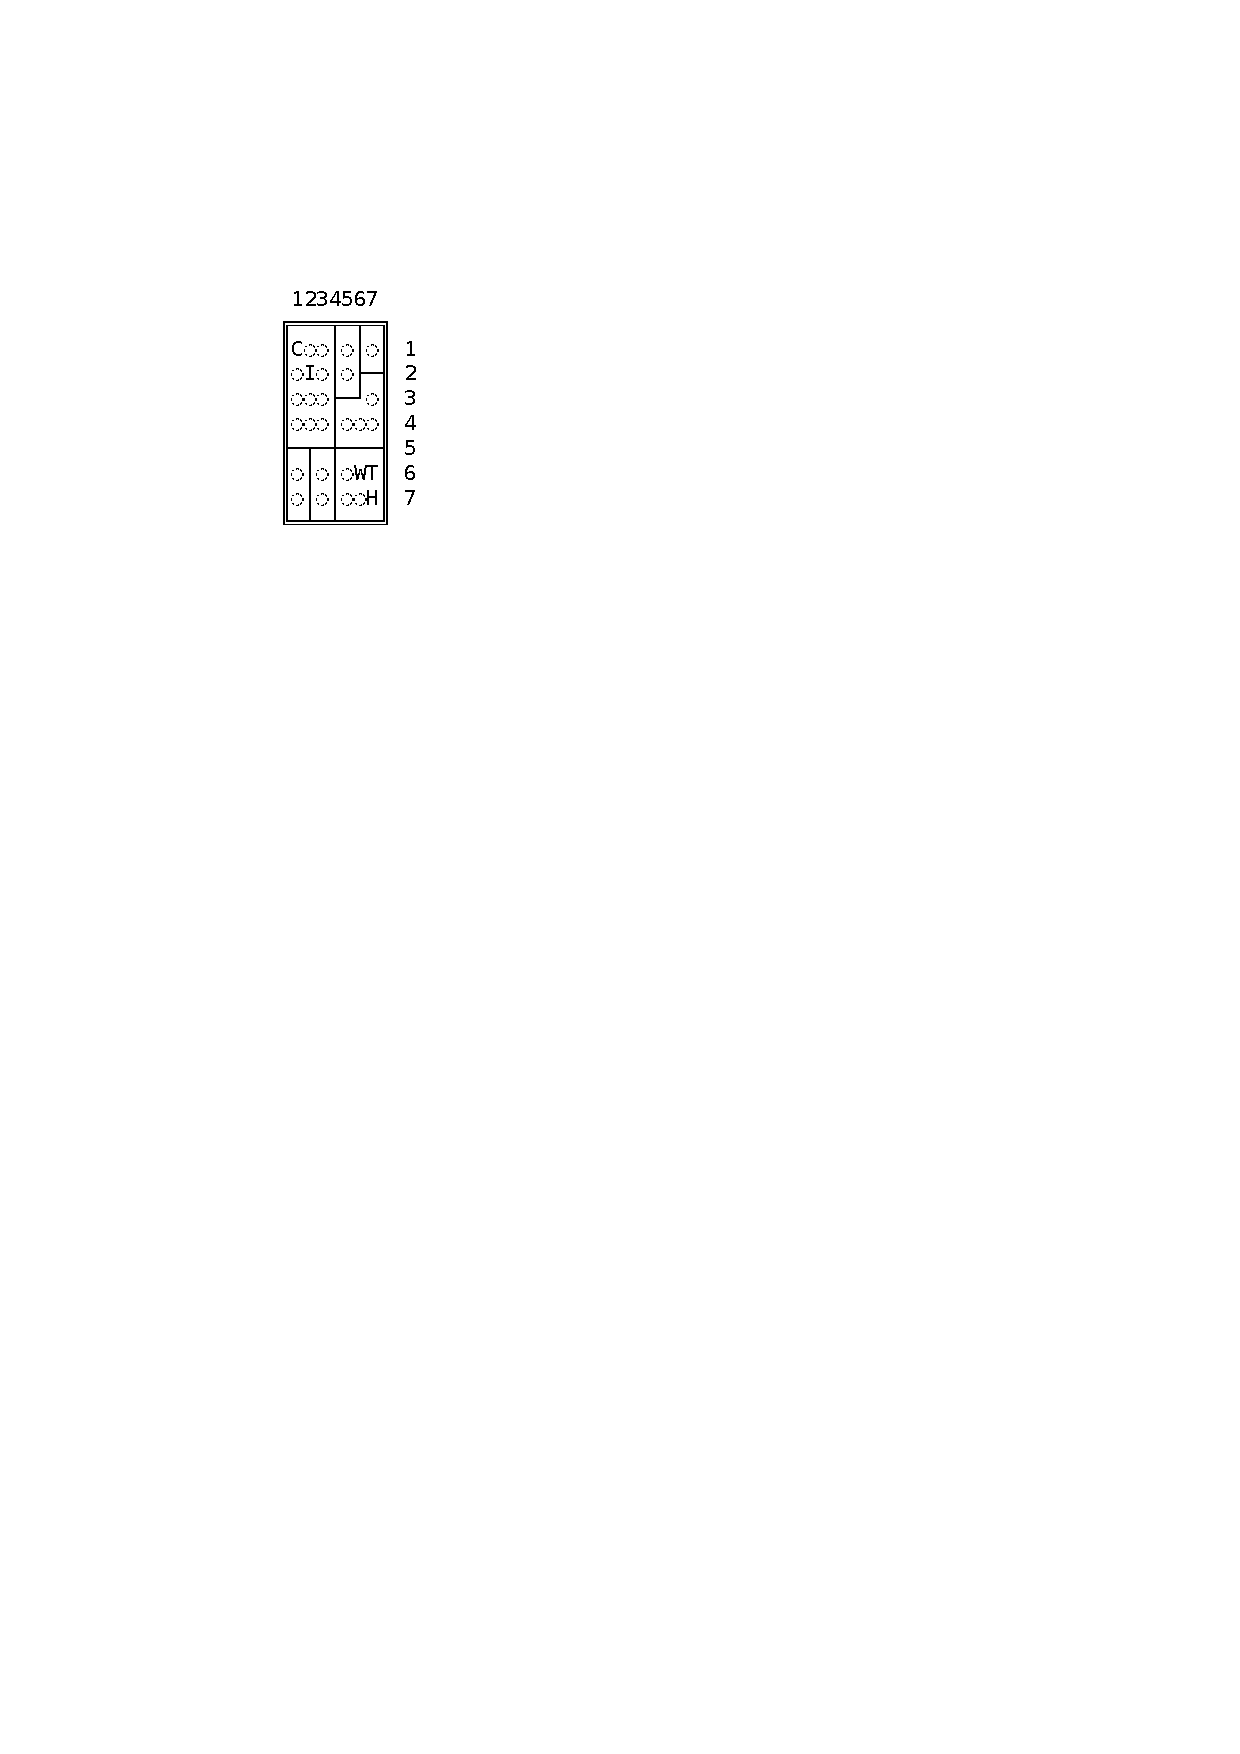
\includegraphics[height=60pt]{clean_up/grid_1_min.pdf}\\
                \raggedright
                \texttt{Please send a message to the other player to start the game!}
            }
        }
    }
    & \\

\theutterance \stepcounter{utterance}  
    & \multicolumn{4}{p{0.6\linewidth}}{
        \cellcolor[rgb]{0.561,0.737,0.561}{
            \makecell[{{p{\linewidth}}}]{
                \texttt{\tiny{[P1$\rangle$GM]}}
                \texttt{SAY: Hi! Let's coordinate our moves. [...]}
            }
        }
    }
    & & \\

\theutterance \stepcounter{utterance}  
    & & \multicolumn{4}{p{0.6\linewidth}}{
        \cellcolor[rgb]{0.9,0.9,0.9}{
            \makecell[{{p{\linewidth}}}]{
                \texttt{\tiny{[GM$\rangle$P2]}}
                \centering{<GAME DESCRIPTION>}\\
                \centering
                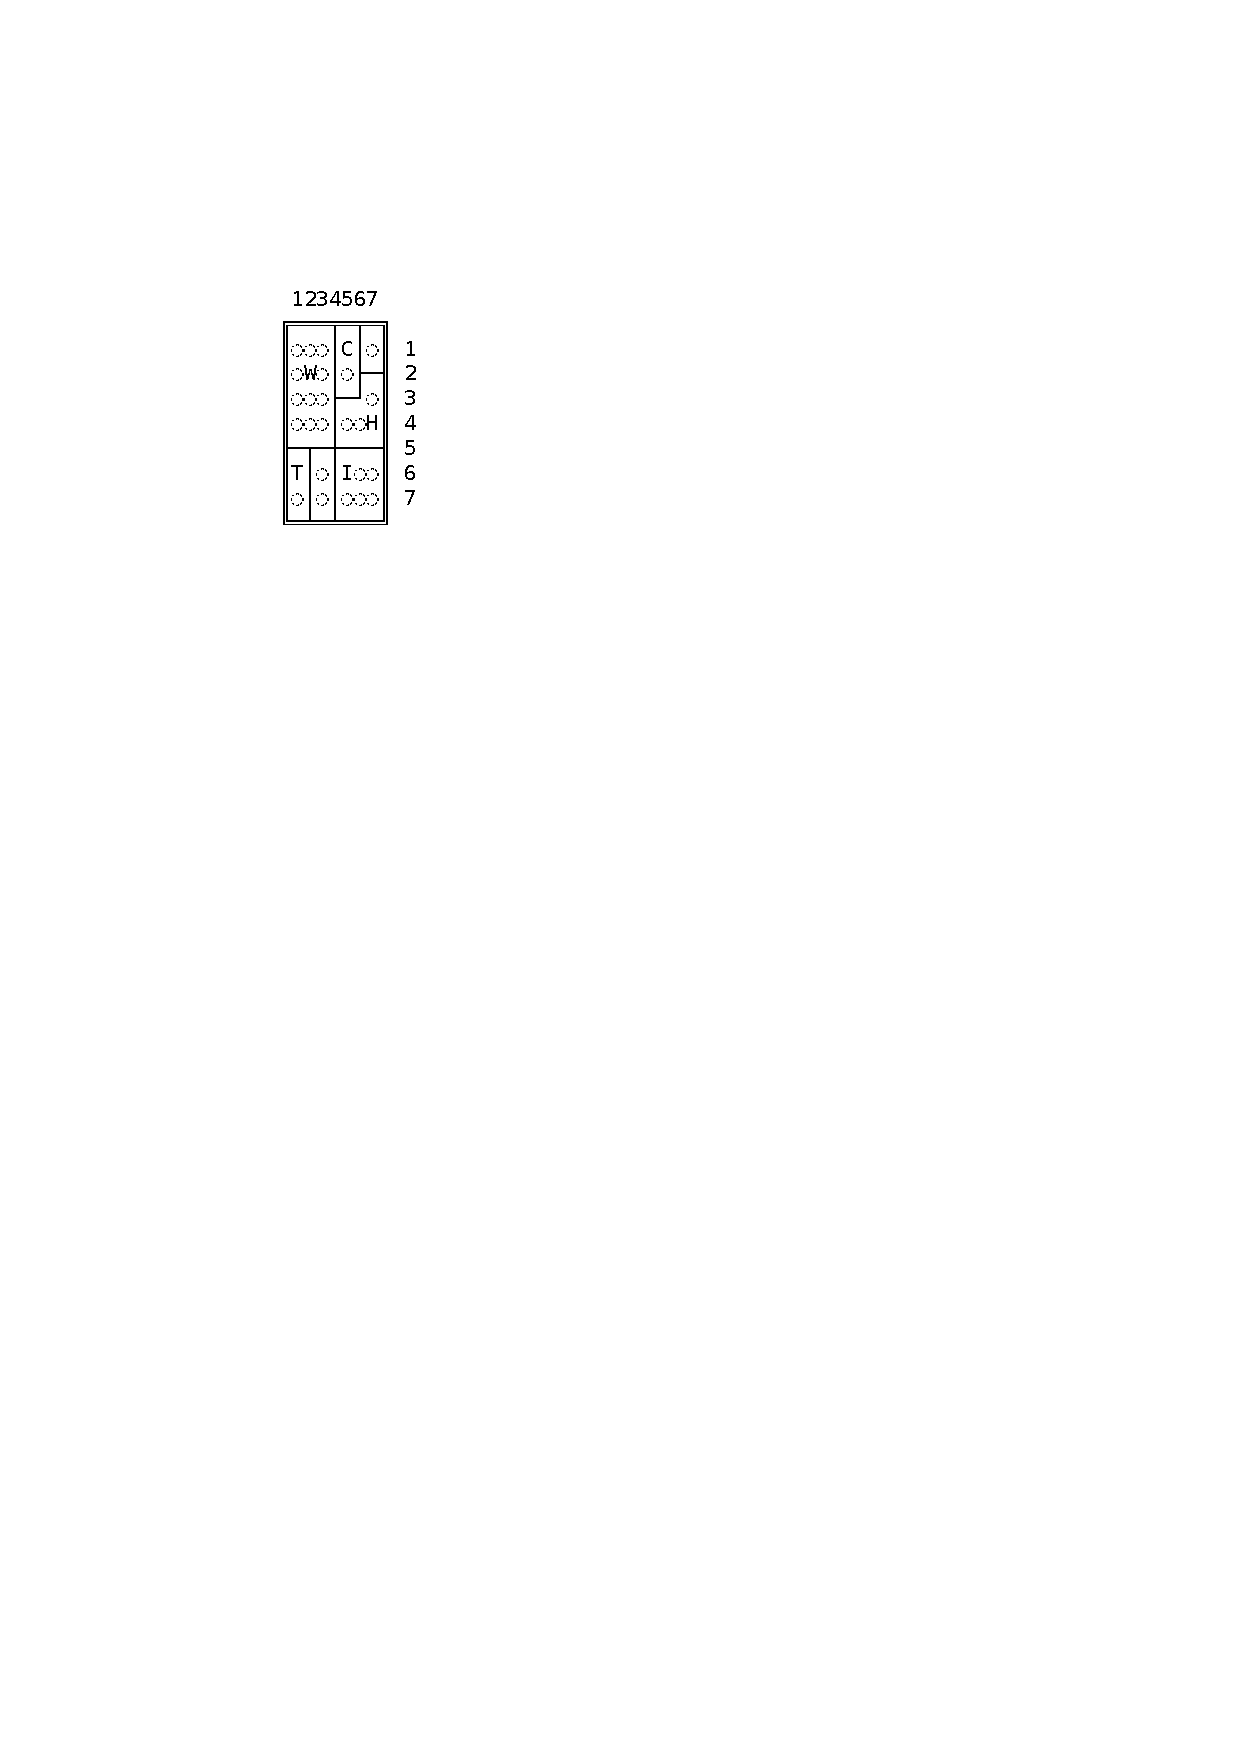
\includegraphics[height=60pt]{clean_up/grid_2_min.pdf}\\
                \raggedright
                \texttt{The other player started the game by sending this message:} \\
                \centering{<MESSAGE>}\\
                \raggedright
                \texttt{What is your first command?}
            }
        }
    }
    & \\

& \multicolumn{6}{c}{
\vdots
} \\

\theutterance \stepcounter{utterance}  
    & & & \multicolumn{4}{p{0.6\linewidth}}{
        \cellcolor[rgb]{0.373,0.62,0.627}{
            \makecell[{{p{\linewidth}}}]{
                \texttt{\tiny{[GM$\langle$P2]}}
                \texttt{MOVE: C, (1,1)} \\
            }
        }
    } \\

\theutterance \stepcounter{utterance}  
    & & \multicolumn{4}{p{0.6\linewidth}}{
        \cellcolor[rgb]{0.9,0.9,0.9}{
            \makecell[{{p{\linewidth}}}]{
                \texttt{\tiny{[P1$\langle$GM]}}
                Your message has been relayed to the other player.\\
                \centering <GAME STATE> \\
                \raggedright
                \texttt{The other player moved an object on their grid. \\What is your next command?}
            }
        }
    }
    & \\
    
\theutterance \stepcounter{utterance}  
    & \multicolumn{4}{p{0.6\linewidth}}{
        \cellcolor[rgb]{0.561,0.737,0.561}{
            \makecell[{{p{\linewidth}}}]{
                \texttt{\tiny{[P1$\rangle$GM]}}
                \texttt{MOVE: I, (5,6)}
            }
        }
    }
    & & \\

& \multicolumn{6}{c}{
    \vdots
} \\
\theutterance \stepcounter{utterance}  
    & & & \multicolumn{4}{p{0.6\linewidth}}{
        \cellcolor[rgb]{0.373,0.62,0.627}{
            \makecell[{{p{\linewidth}}}]{
                \texttt{\tiny{[GM$\langle$P2]}}
                \texttt{SAY: I think our grids are aligned now, finished?} \\
            }
        }
    } \\
\theutterance \stepcounter{utterance}  
    & \multicolumn{4}{p{0.6\linewidth}}{
        \cellcolor[rgb]{0.561,0.737,0.561}{
            \makecell[{{p{\linewidth}}}]{
                \texttt{\tiny{[P1$\rangle$GM]}}
                \texttt{SAY: finished!}
            }
        }
    }
    & & \\
\end{supertabular}